\chapter{Especificación del Problema}

% Descripción detallada del problema a resolver
% Se discute la relevancia de contar con una solución
% Se especifica en todo detalle los requisitos de la solución a construir
% Características de calidad de la solución deseada
% Es deseable también establecer criterios de aceptación de una solución al problema

\section{Descripción del problema}

El problema a resolver, esencialmente, es el de encontrar reglas de asociacion entre líneas moleculares detectadas en espectros de frecuencia obtenidos a partir de observaciones astronómicas.

Para ello, se asume que las líneas ya han sido detectadas en los distintos espectros; vale decir, se sabe que están presentes y se conocen sus posiciones dentro del rango de frecuencias. En la práctica eso puede ser muy difícil de lograr, sobre todo en circunstancias donde potencialmente pueden existir una alta cantidad de líneas espectrales y estas pueden interferir unas con otras en la señal final, lo que se conoce como \textit{blending}. 

Sin embargo, no es necesario que todas las líneas se encuentren ya identificadas; vale decir, que se sepa a qué especie (átomo, molécula, etc.) se encuentran asociadas. Actualmente existen herramientas que son capaces de ajustar modelos físicos conocidos con anterioridad a datos espectrales con el fin de identificar las líneas en ellos presentes.

\section{Requisitos de la solución y casos de uso}

A continuación se enuncian los requerimientos del sistema:

\begin{enumerate}
	\item \textbf{Obtener reglas de asociación entre líneas de emisión espectrales [esencial].} \\
	El sistema debe generar reglas de asociación entre líneas de emisión presentes en espectros, independientemente de si estos pertenecen a una misma o a distintas moléculas o átomos, o si no han sido aun identificadas.
	\item \textbf{Permitir al usuario observar las reglas generadas, y desplegarlas a este ordenadas según distintas medidas de relevancia [esencial].} \\
	\item \textbf{Permitir al usuario guardar las reglas de asociación generadas [esencial].} \\
	Una vez extraídas las reglas de asociación, el usuario debe poder revisarlas y guardarlas para su revisión posterior.
	\item \textbf{Permitir al usuario aplicar los mismos algoritmos de reglas de asociación a datos de diversas fuentes [esencial].} \\
	Se desea que el sistema de extracción sea lo más general posible, de modo tal de poder aplicarlo a datos de líneas espectrales extraídos de distintos \textit{surveys}, bases de datos, sistemas de modelamiento y detección de líneas, entre otros.
	\item \textbf{El sistema debe ser ejecutable en un ambiente de computación de alto rendimiento [deseable].}
	\item \textbf{El sistema debe ser compatible con plataformas de observatorios virtuales [deseable].} 
	\item \textbf{Implementar una interfaz gráfica de usuario [opcional].}
\end{enumerate}

\subsection{Casos de Uso}

En la Figura \ref{fig:cases} se muestra un diagrama con los casos de uso preliminares del sistema a desarrollar, y a continuación se describen estos en detalle junto con sus actores.

\begin{figure}[h!]
\begin{center}
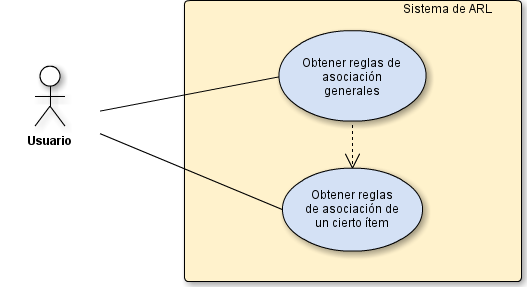
\includegraphics[width=0.9\textwidth]{imagenes/casos_de_uso.png}
\end{center}
\vspace*{-5mm}
\caption{Diagrama de casos de uso del sistema.}
\label{fig:cases}
\end{figure}

\subsubsection{Actores}

Para este sistema existe solo un tipo de actor, dado que todos los usuarios finales tendrán acceso a las mismas funcionalidades. Este usuario será el encargado de seleccionar el conjunto de datos que quiere ingresar al sistema, en forma de transacciones de líneas moleculares. Cada transacción poseerá las líneas identificadas en un espectro en particular. Este usuario ingresará estos datos al sistema y luego seleccionará los parámetros de detección de reglas que desee. Una vez ejecutados los algoritmos correspondientes, el usuario podrá observar las reglas generadas y, si así lo desea, ajustar nuevamente los parámetros para obtener mejores resultados sobre el mismo conjunto de datos.

Desde un punto de vista práctico, el usuario objetivo posee conocimientos técnicos sobre espectroscopía, sabe hacer uso de un terminal o línea de comandos, y puede manejar tablas en formato de valores separados por comas (CSV).


\subsubsection{Descripción de casos de uso}

En la siguiente tabla se muestra una descripción detallada de los casos de uso y se indica, de ser así, a qué requerimiento está asociado.

\begin{tabular}{|l|p{4cm}|p{7cm}|l|l|}
	\hline
	ID & Caso de uso & Descripción & Tipo & Ref. \\ \hline
	1 & Obtener reglas de asociación generales & El usuario obtiene reglas de asociación extraídas a partir de un conjunto de transacciones de líneas espectrales y las filtra u ordena mediante soporte, confianza o \textit{lift} & Esencial & 1,2,3,4 \\ \hline
	2 & Obtener reglas de asociación de un cierto ítem & El usuario obtiene reglas de asociación extraídas a partir de un conjunto de transacciones de líneas espectrales, selecciona solo aquellas que posean un cierto ítem en su antecedente y/o consecuente, y las ordena mediante soporte, confianza o \textit{lift}. & Esencial & 1,2,3,4 \\ \hline
\end{tabular}
